% Template for ICASSP-2010 paper; to be used with:
%          mlspconf.sty  - ICASSP/ICIP LaTeX style file adapted for MLSP, and
%          IEEEbib.bst - IEEE bibliography style file.
% --------------------------------------------------------------------------
\documentclass{article}
\usepackage{amsmath,graphicx,mlspconf}
\usepackage{amsfonts}
\usepackage{tikz}
\usetikzlibrary{shapes,arrows,positioning,calc}

%Select one of the four copyright notices below. Only required for the camera paper submission

%For papers in which all authors are employed by the US government, the copyright notice is:
\copyrightnotice{U.S.\ Government work not protected by U.S.\ copyright}

%For papers in which all authors are employed by a Crown government (UK, Canada, and Australia), the copyright notice is:
\copyrightnotice{978-1-5090-6341-3/17/\$31.00 {\copyright}2017 Crown}

%For papers in which all authors are employed by the European Union, the copyright notice is:
\copyrightnotice{978-1-5090-6341-3/17/\$31.00 {\copyright}2017 European Union}

%For all other papers the copyright notice is:
\copyrightnotice{978-1-5090-6341-3/17/\$31.00 {\copyright}2017 IEEE}

\toappear{2017 IEEE International Workshop on Machine Learning for Signal Processing, Sept.\ 25--28, 2017, Tokyo, Japan}


% Example definitions.
% --------------------
\def\x{{\mathbf x}}
\def\L{{\cal L}}

% Title.
% ------
\title{A Neural Network Alternative to Convolutive Audio Models for Source Separation}
%
% Single address.
% ---------------
\name{Author(s) Name(s) omitted for double blind review\thanks{Thanks to XYZ agency for funding.}}
\address{Author Affiliation(s) omitted for double blind review}
%
% For example:
% ------------
%\address{School\\
%	Department\\
%	Address}
%
% Two addresses (uncomment and modify for two-address case).
% ----------------------------------------------------------
%\twoauthors
%  {A. Author-one, B. Author-two\sthanks{Thanks to XYZ agency for funding.}}
%	{School A-B\\
%	Department A-B\\
%	Address A-B}
%   Email A-B
%  {C. Author-three, D. Author-four\sthanks{The fourth author performed the work
%	while at ...}}
%	{School C-D\\
%	Department C-D\\
%	Address C-D
%   Email C-D}
%


\tikzset{
block/.style = {draw, fill=white, rectangle, minimum height=3em, minimum width=3em},
tmp/.style  = {coordinate}, 
sum/.style= {draw, fill=white, circle, node distance=1cm},
input/.style = {coordinate},
output/.style= {coordinate},
pinstyle/.style = {pin edge={to-,thin,black}
}
}

\begin{document}
%\ninept
%

\maketitle
%
\begin{abstract}
We present a convolutiional auto-encoder that can act as a neural network equivalent to convolutive audio models. We demonstrate the ability of the network to learn optimal bases that resemble phoneme magnitude-spectra and also show how it can be used for supervised separation of speech mixtures. In terms of separation performance, the ability of the network to learn cross-frame characteristics from input spectrograms enables these models to significantly outperform their feed-forward counterpart. More importantly, we can now exploit the available diversity of neural networks to propose novel and potentially powerful extensions to existing auto-encoder architectures, based on a cascade of recurrent and convolutional neural network layers. 

\end{abstract}
%
\begin{keywords}
Auto-encoders, source separation, deep learning, convolutive models.
\end{keywords}
%
\section{Introduction}
\label{sec:intro}

% Several neural network architectures have been proposed to develop algorithms for supervised source separation and speech enhancement~\cite{chandna2017monoaural,grais2017single, venkataramani2017end, park2016fully}. Currently, these networks are trained to learn discriminative audio models extensively. In other words, the spectrogram of the mixture is given as an input to the network. The goal of the network then, is to learn suitable time-frequency masks that separate the input spectrogram into the source and the interference components. Thus, the networks learn a basis decomposition that often works only for a specific source-interference pair, i.e., these models are not transferable. If the interfering signal changes, these networks have to be re-trained to learn suitable models to separate the new interfering signal in the mixture from the source. \textbf{Cem: I am not sure if starting the paper with a generative vs discriminative (transferability) discussion is the right way. }  \\



Non-negative matrix factorization~(NMF) of magnitude-spectrograms has been a very popular method for modeling sources for supervised source separation applications~\cite{smaragdis2014static, virtanen2015compositional}. NMF factorizes a matrix of non-negative elements~$\mathbf{X}\in \mathbb{R}_{M\times N}^{\geq0}$ as a product of the basis matrix~$\mathbf{W}$ and the activation matrix~$\mathbf{H}$. The notation $\mathbb{R}_{M \times N}^{\geq0}$ represents the set of matrices of non-negative elements of size $M \times N$. In this factorization, the basis matrix $\mathbf{W} \in \mathbb{R}_{M \times r}^{\geq{0}}$, the activation matrix $\mathbf{H} \in \mathbb{R}_{r \times N}^{\geq{0}}$ and $r$ represents the rank of the decomposition. In the case of audio signals, we apply NMF on audio spectrograms. In the audio setting, the columns of $\mathbf{W}$ begin to act as representative basis vectors for the source. The rows of $\mathbf{H}$ indicate the activity of these basis vectors in time. \textbf{Cem: I am not sure how smooth the transition to neural nets here.} As shown in~~\cite{smaragdis2017aneural}, the notion of non-negative audio modeling can be easily generalized by interpreting NMF as a neural network. We can interpret NMF as a non-negative auto-encoder in the following manner,
\begin{align}
    \text{$1^{\text{st}}$ layer:~}\mathbf{H} &= g(\mathbf{W^{\ddagger}} \cdot \mathbf{X}) \\
    \text{$2^{\text{nd}}$ layer:~}\mathbf{X} &= g(\mathbf{W} \cdot \mathbf{H})
    \label{eq:nmfae}
\end{align}

Here, $\mathbf{X}$ represents the input spectrogram, $\mathbf{W^{\ddagger}}$ represents a form of pseudo-inverse of $\mathbf{W}$ and $g(.):\mathbf{R}\rightarrow \mathbf{R}^{\geq0}$ is an element-wise function that maps a real number to the space of positive real numbers. As before, the columns of $\mathbf{W}$ act as representative basis vectors and the corresponding rows of $\mathbf{H}$ indicate their respective activations. Although non-negativity of the network-parameters (models) is not explicitly guaranteed in this formulation, applying a suitable sparsity constraint allows the network to learn suitable non-negative models. Additionally, this interpretation enables a pathway to propose multi-layer extensions by exploiting the wealth of available neural net architectures that could potentially lead to superior separation performance.

Spectrograms of speech and audio signals incorporate temporal dependencies that span multiple time frames. However, NMF and its neural network equivalent are unable to explicitly utilize these cross-frame patterns available in a spectrogram. To alleviate this drawback, Smaragdis~\cite{smaragdis2007convolutive} proposed a convolutive version to NMF~(conv-NMF) that allows spectro-temporal patterns as representative basis elements. In this paper, we develop a neural network alternative to such convolutive audio models for supervised source separation. In doing so, we solve two fundamental problems associated with this task. The first step is to develop a suitable neural network architecture to learn convolutive audio models in an adaptive manner. Utilizing the models to separate a source from a given mixture forms the second step. 

Developing a neural network alternative to conv-NMF also results in a significant advantage in terms of model re-usability. Several neural network architectures have been recently proposed for supervised source separation~\cite{grais2017single, venkataramani2017end}. These networks are trained to learn discriminative audio models by training them on mixture spectrograms. Thus, the networks learn a decomposition that works only for a specific source-interference pair. Developing an alternative to conv-NMF allows us to learn audio-models by training neural networks on clean source spectrograms. These models can be easily re-used irrespective of the interfering component. The remainder of the paper is organized as follows. In section~\ref{sec:}, we develop an auto-encoder that can act as an equivalent to conv-NMF audio models. Section~\ref{sec:} proposes a novel approach to utilize these models for supervised source separation. We evaluate these models in terms of their separation performance in section~\ref{sec:} and conclude in section~\ref{cite:}.

\begin{figure}[t]
\centering
  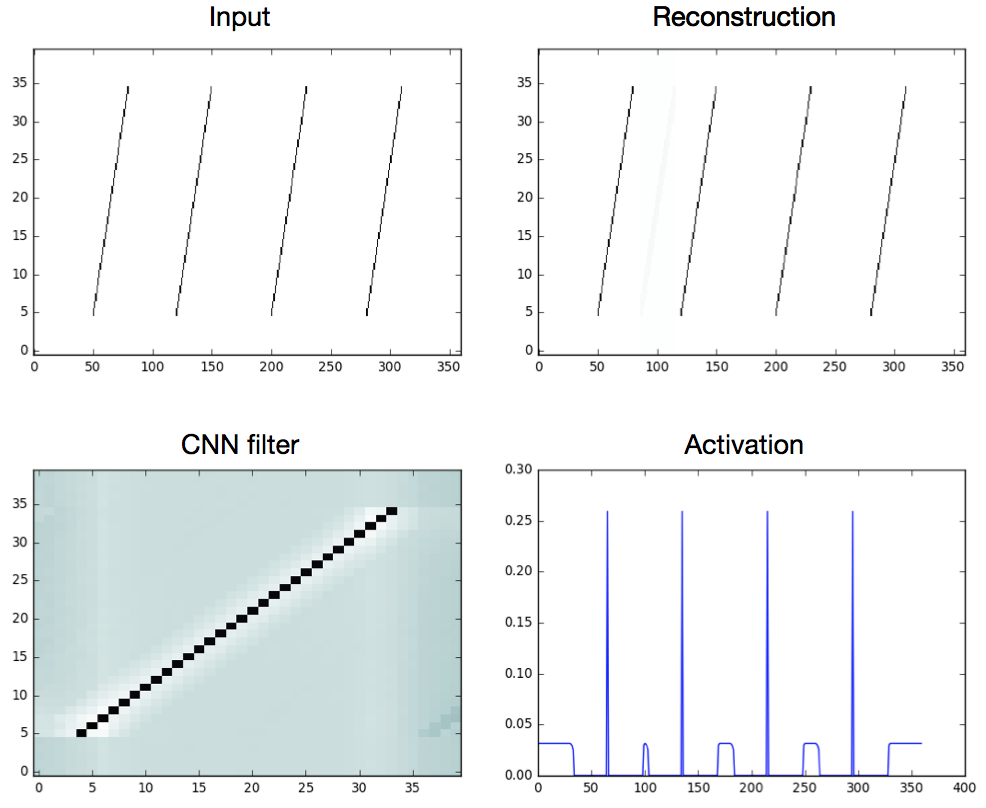
\includegraphics[clip, trim = 0cm 0cm 0cm 0cm, width=\linewidth]{Figs/CNN_demo.png}
  \caption{Basis decomposition of a toy-illustration obtained using a CNN-CNN auto-encoder.}~\label{fig:cnn_demo}
\end{figure}

\section{Non-negative Convolutional Auto-encoders}
\subsection{Network Architecture}
\label{sec:conv-nmf}
The convolutive NMF model~\cite{smaragdis2007convolutive} approximates a non-negative matrix~$\mathbf{X}\in \mathbb{R}_{M \times N}^{\geq0}$ as,
\begin{equation}
    \mathbf{X}(f,t) \approx \sum_{i=1}^{r} \sum_{k=0}^{T-1} \mathbf{W}_{i}(k,f)\cdot\mathbf{H}(i,t-k)
\end{equation}
Here, $\mathbf{W}_{i} \in \mathbb{R}_{M \times T}^{\geq0}$ acts as the $i^{\text{th}}$ basis matrix and $\mathbf{H} \in \mathbb{R}_{r \times N}^{\geq0}$ contains the corresponding weights. The notation $\mathbf{X}(i,j)$ represents the element of $\mathbf{X}$ indexed by the $i^{\text{th}}$ row and the $j^{\text{th}}$ column. We can interpret this operation as a two-layer convolutional auto-encoder~(CAE) as follows,

\begin{align}
  \text{$1^{st}$ layer:~}\mathbf{H}(i,t) &= \sum_{j=0}^{M-1} \sum_{k=0}^{T-1} \mathbf{W}_{i}^{\ddagger}(j,k)\mathbf{X}(j,t-k) \\
  \text{$2^{nd}$ layer:~}\hat{\mathbf{X}}(f,t) &= \sum_{i=1}^{r} \sum_{k=0}^{T-1} \mathbf{W}_{i}(k,f)\cdot\mathbf{H}(i,t-k)
    \label{eq:nmfcnncnn}
\end{align}
subject to non-negativity of $\mathbf{W}_{i}$ and $\mathbf{H}$. Here, we assume that the convolutional layer filters~$\mathbf{W},~\mathbf{W}^{\ddagger}$ have a size of $M\times T$ where, $T$ represents the depth of the convolution and $M$ denotes the height of the input matrix~$\mathbf{X}$. In this representation, $\mathbf{W}_{i}$ and $\mathbf{H}$ correspond to the $i^{\text{th}}$ basis matrix and the activation matrix respectively. The filters of the first convolutional neural network~(CNN) act as inverse filters in defining the auto-encoder. In the remainder of this section, we will refer to the first convolutional layer as the ``encoder'' that estimates a code from the input representation. The second CNN layer generates an approximation of the input from the code and will be referred to as the ``decoder''. We can satisfy the non-negativity constraints by incorporating a non-linearity into the definitions of the encoder and the decoder. Thus,

\begin{align}
    \text{$1^{\text{st}}$ layer:~}\mathbf{H}(i,t) &= g\left(\sum_{j=0}^{M-1} \sum_{k=0}^{T-1} \mathbf{W}_{i}^{\ddagger}(j,k)\mathbf{X}(j,t-k)\right) \\
    \text{$2^{\text{nd}}$ layer:~}\hat{\mathbf{X}}(f,t) &= g\left(\sum_{i=1}^{r} \sum_{k=0}^{T-1} \mathbf{W}_{i}(k,f)\cdot\mathbf{H}(i,t-k)\right)
    \label{eq:nmfcnncnn}
\end{align}

Here, the $g(.):\mathbb{R}\rightarrow \mathbb{R}^{\geq0}$ applies an element-wise non-linearity and ensures that the activation matrix and the reconstruction are non-negative. The block diagram of the whole CNN-CNN encoder is given in Figure \ref{diag:cnncnn}. In our experiments, we used the soft-plus function which is given by the formula $g(x) = \log(1+\exp(x))$ as the non-linearity. We now note some key points about the CAE. (i) The output of the encoder gives the latent representation (analog of activations in NMF \textbf{cem:we do not give the reference to corresponding equation number here} of the decomposition. (ii) The weights of the decoder act as the basis vectors of the decomposition. (iii) We do not explicitly apply non-negativity constraints on the weights. Thus, the basis matrices (decoder filters) can assume negative values. To train the auto-encoder, we minimize the KL-divergence between the input spectrogram~$\mathbf{X}$ and its reconstruction~$\hat{\mathbf{X}}$ given by,
\begin{equation*}
    D\left(\mathbf{X},\hat{\mathbf{X}}\right) = \sum_{i,j} \mathbf{X}(i,j)\cdot \text{log}\frac{\mathbf{X}(i,j)}{\hat{\mathbf{X}}(i,j)} - \mathbf{X}(i,j) + \hat{\mathbf{X}}(i,j)
\end{equation*}


\begin{figure*}[t]
  \centering
  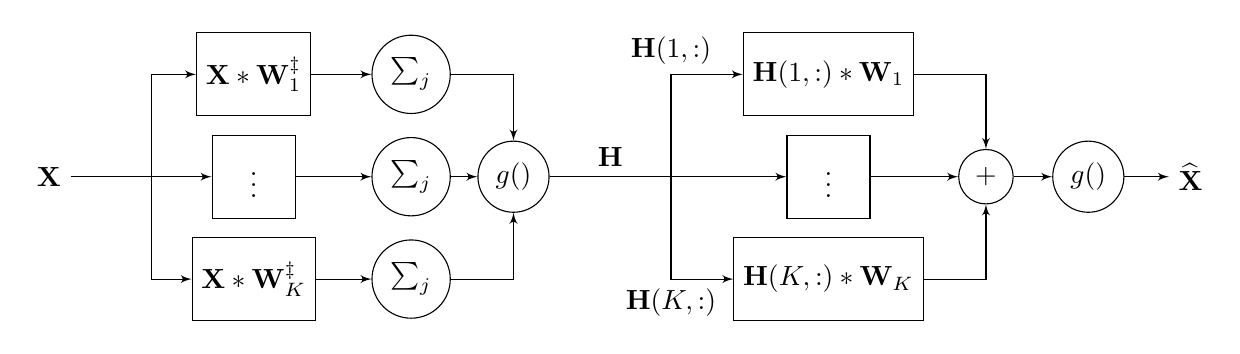
\begin{tikzpicture}[auto, node distance=2cm,>=latex']
      
      \node [,name=input] (input) {$\mathbf X$};
      \coordinate [, name=rinput, right of=input, node distance=1.3cm ](rinput) {};
      \node [block, right of=rinput, node distance=1.3cm] (controller) {$\vdots$};
      \node [sum, right of=controller, node distance=2cm] (controllers){$\sum_j$};
      \node [block, above of=controller,node distance=1.3cm] (up){$\mathbf X *\mathbf W^\ddagger_1$};
      \node [sum, right of=up, node distance=2cm] (ups) {$\sum_j$};
      \node [block, below of=controller,node distance=1.3cm] (rate) {$\mathbf X*\mathbf W^\ddagger_K$};
      \node [sum, right of=rate, node distance=2cm] (rates) {$\sum_j$};	

      \node [sum, right of=controllers,node distance=1.3cm] (sum2) {$g()$};
      \coordinate[, right of=sum2,node distance=2cm] (system) {};
      \node [block, right of=system, node distance=2cm] (dec2) {$\vdots$};
      \node [block, above of=dec2, node distance=1.3cm] (dec1) {$\mathbf H(1, :) * \mathbf W_1$};
      \node [block, below of=dec2, node distance=1.3cm] (dec3) {$\mathbf H(K, :) *\mathbf W_K$};
      \node [sum, right of=dec2, node distance=2cm] (sum3) {$+$};
      \node [sum, right of=sum3, node distance=1.3cm] (g2) {$g()$};
      \node [,right of=g2, node distance=1.3cm] (outp) {$\widehat{\mathbf X}$};

      \draw [-] (input) -- (rinput);
      \draw [->] (rinput) -- (controller); 
      \draw [->] (controller) -- (controllers);
      \draw [->] (controllers) -- (sum2);
      \draw [-] (sum2) --node{$\mathbf H$} (system);
      \draw [->] (rinput) |- (rate);
      \draw [->] (rate) -- (rates);
      \draw [->] (rates) -| (sum2);
      \draw [->] (rinput) |- (up);
      \draw [->] (up) -- (ups);
      \draw [->] (ups) -| (sum2);
      \draw [->] (system) -- node {} (dec2);
      \draw [->] (system) |- node {$\mathbf H(1,:)$} (dec1);
      \draw [->] (system) |- node[anchor=north]{$\mathbf H(K,:)$} (dec3);
      \draw [->] (dec1) -| (sum3);
      \draw [->] (dec2) -- (sum3);
      \draw [->] (dec3) -| (sum3);
      \draw [->] (sum3) -- (g2);
      \draw [->] (g2) -- (outp);
    \end{tikzpicture}
  \caption{Block Diagram of CNN-CNN Autoencoder} 
  \label{diag:cnncnn}
\end{figure*}



\begin{figure}[ht!]
\centering
  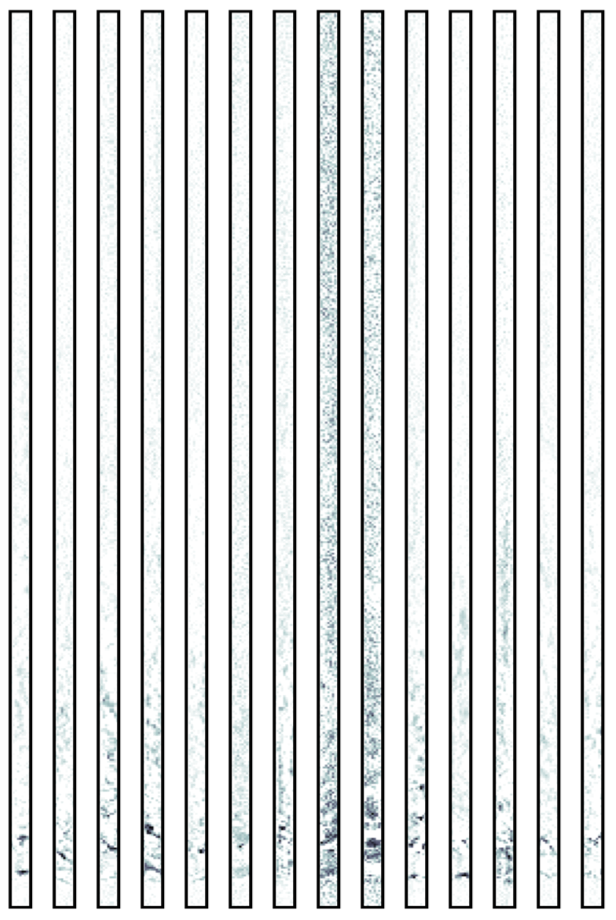
\includegraphics[clip, trim = 0cm 0cm 0cm 0cm, width=\columnwidth, height = \columnwidth]{Figs/Bases.png}
  \caption{A subset of decoder filters obtained by training the CAE on magnitude-spectrograms of utterances of a male speaker. This decomposition is obtained for the configuration $K = 80$ and $T = 8$. We see that the filters resemble snippets of a speech spectrogram.}~\label{fig:cnn_demo_speech}
\end{figure}
Although the filters can assume negative values, the use of a non-linearity does not allow cross-cancellations across the basis elements.  



\subsection{Practical Considerations}
\label{subsec:practical}
Having developed the CAE equivalent to conv-NMF, we can now begin to understand the nature of the basis and activation matrices learned by the network. To do so, we train the convolutive auto-encoder defined by~(\ref{eq:nmfcnncnn}) on a simple toy example as shown in figure~\ref{cnn_demo}. We also incorporate sparsity constraints on the activation, i.e., the output of the first CNN. In this example, the CNN filter resembles a snippet of the input spectrogram. We also see that the activation comprises a series of impulse trains. Thus, the encoder acts as a matched-filter and identifies the points in time when the corresponding pattern becomes active. As shown in (\ref{eq:nmfcnncnn}), the time-frequency pattern is captured by the filters of the decoder. Given the nature of the activation we see that the encoder attempts to learn the inverse filter to the decoder. Figure~\ref{fig:cnn_demo_speech} shows the decoder filters obtained by training the CAE on speech utterances of a male speaker. Similar to the previous toy-example, the decoder filters learn patterns that resemble snippets of a speech spectrogram. 

\textbf{Cem: Impulse response concept is for linear systems. I am not too sure about using it in this context.} The decoder CNN can be interpreted as a finite impulse response~(FIR) filter. The encoder attempts to approximate the inverse of the decoder FIR filter as an FIR filter. From our knowledge of signal processing, it can be shown that the inverse filter of an FIR filter has an infinite impulse response~(IIR)~\cite{} (**Give reference**). Thus, approximating the encoder as an FIR filter or a CNN will hinder the decoder from learning patterns that are invertible only by an IIR filter. One such example is shown in figure~\ref{fig:}. Therefore, we explore using a Recurrent Neural Network~(RNN) to get an IIR encoder.

\section{Using a recurrent filter in the encoder}
\label{sec:rnncnn}

%As discussed above, the encoder part acts as the inverse filter to the decoder. We can think of a CNN as a filter with a finite impulse response. As known from DSP theory, the inverse of an FIR filter is an IIR filter. To the best of our knowledge, this results in a novel RNN-CNN auto-encoder architecture. In the remainder of the paper, we will refer to this auto-encoder as a Recurrent-Convolutive Auto-encoder~(RCAE). 

In this section, the goal is to construct a recurrent encoder analogous to the convolutive encoder we discussed in the previous section. The potential gain of using a recurrent encoder over a finite length convolutive encoder is due to the fact that a recurrent filter in theory can capture arbitrarily long temporal dependencies. From a signal processing point of view, the motivation for going with a recurrent filter is that, the inverse of an finite length filter (the convolutive basis in the encoder) is given by a recurrent filter. We explore the idea, and obtain source separation results on the same dataset.  

The way we go about building an encoder is by passing the input through $K$ separate recurrent neural networks (RNNs) (Note that $K$ was the number of filters/components in the convolutive model). The $k$'th RNN recursion in the encoder is given by the following equation:    

\begin{align}
  \mathbf Z(k_1, t, k) =& \tanh \Bigg( \sum_{k_2 = 1}^{K_{in}} \mathbf W^k(k_1,k_2 ) \mathbf Z(k_2, t-1, k) + \notag \\
  & \hspace{0cm} \sum_l \mathbf U^k(k_1,l) \mathbf X(l, t) \Bigg),\; k \in \{1,\dots,K\}, 
\end{align}
where $\mathbf Z(:, t, k) \in \mathbb R^{K_{in}}$ denotes the latent state vector of the $k$'th RNN at time $t$. We denote the hidden state dimensionality of each RNN with $K_{in}$. The recurrent and projection matrices of the $k'th$ RNN are respectively denoted with $\mathbf W^k$, and $\mathbf U^k$. Note that although the given recursion corresponds to the vanilla-RNN architecture, there is no restriction on the RNN architecture choice. In our experiments, we have used the LSTM architecture [cite]. After going through the RNN recursions, the encoder output $\mathbf H(i, t)$ is obtained by summing the RNN outputs over the first dimension:
\begin{align}
  \mathbf H(i, t) = \sum_{k_1=1}^{K_{in}} \mathbf Z(k_1, t, i)
\end{align}

The recurrent encoder's block diagram is given in Figure \ref{diag:rnnenc}. 

\begin{figure*}[t]
  \centering
  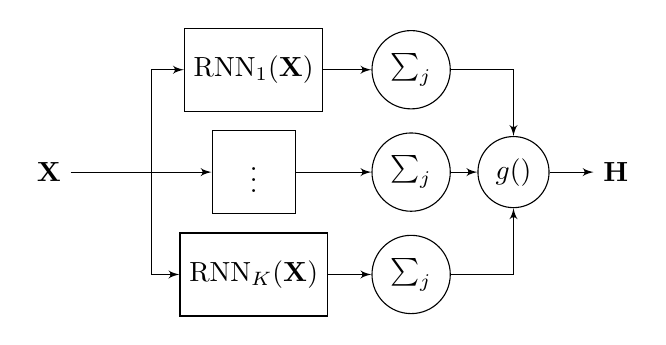
\begin{tikzpicture}[auto, node distance=2cm,>=latex']
      
      \node [,name=input] (input) {$\mathbf X$};
      \coordinate [, name=rinput, right of=input, node distance=1.3cm ](rinput) {};
      \node [block, right of=rinput, node distance=1.3cm] (controller) {$\vdots$};
      \node [sum, right of=controller, node distance=2cm] (controllers){$\sum_j$};
      \node [block, above of=controller,node distance=1.3cm] (up){$\text{RNN}_1(\mathbf X)$};
      \node [sum, right of=up, node distance=2cm] (ups) {$\sum_j$};
      \node [block, below of=controller,node distance=1.3cm] (rate) {$\text{RNN}_K(\mathbf X)$};
      \node [sum, right of=rate, node distance=2cm] (rates) {$\sum_j$};	

      \node [sum, right of=controllers,node distance=1.3cm] (sum2) {$g()$};
      \node[, right of=sum2,node distance=1.3cm] (system) {$\mathbf H$};
      
      \draw [-] (input) -- (rinput);
      \draw [->] (rinput) -- (controller); 
      \draw [->] (controller) -- (controllers);
      \draw [->] (controllers) -- (sum2);
      \draw [->] (sum2) --(system);
      \draw [->] (rinput) |- (rate);
      \draw [->] (rate) -- (rates);
      \draw [->] (rates) -| (sum2);
      \draw [->] (rinput) |- (up);
      \draw [->] (up) -- (ups);
      \draw [->] (ups) -| (sum2);
      \end{tikzpicture}
  \caption{Block Diagram of RNN Encoder} 
  \label{diag:rnnenc}
\end{figure*}




% This is the same as CNN-CNN case, except the computation of the activations $H$. In the CNN encoder, each filter was of finite length. With RNN-CNN version, we are attempting to use an infinite length filter. The computation of $\hat H$ is as follows: 

% \begin{align}
% 	Z(:,k,t) =& \sigma( W Z(:,k,t-1) + U X(:,t)) \notag \\
% 	\hat H(k,t) =& \sum_f Z(f,k,t)
% \end{align}

% Give a toy example which shows what this model can do that CNN-CNN can not. 

% \section{Multi-layer Extensions}
% \label{sec:multlayer}


\section{Supervised Source Separation}
\label{sec:ss}
The problem of supervised source separation is solved as a two-step procedure~\cite{smaragdis2007supervised}. The fist step of the procedure is to learn suitable models for a given source. We refer to this step as the training step. In the second step, we use these models to explain the contribution of the source in an unknown mixture. In section~\ref{sec:conv-nmf}, we have developed the auto-encoder architecture to learn suitable convolutive models for a given source. We now turn our attention to the problem of using the models for separating the source in an unknown mixture.

The previous approach to source separation~\cite{smaragdis2017aneural} using neural-network based audio-models involves estimating the latent representation of the bases, which captures the contribution of the bases to each frame of the mixture spectrogram. This does not utilize the encoder component of the auto-encoder for the separation task. In this paper, we present a novel-separation scheme that utilizes the complete auto-encoder architecture for separation. We do so by using the following setup for separation. 

Given an input spectrogram $\mathbf{X}$, the auto-encoder produces an approximation of the input spectrogram which is a linear combination of its weights. We will denote to this approximation as,
\begin{equation}
    \hat{\mathbf{X}} = Ae(\mathbf{X}|\theta)
    \label{eq:separation_ae}
\end{equation}
Here, $\theta$ denotes the weights (parameters) of the auto-encoder. For the separation procedure, given the trained auto-encoders, (i.e., given $\theta_{1}$ and $\theta_{2}$), the goal is to identify suitable input spectrograms $\mathbf{X}_{1}$ and $\mathbf{X}_{2}$ such that,
\begin{equation}
    \mathbf{X}_{m} = Ae(\mathbf{X}_{1}|\theta_{1}) + Ae(\mathbf{X}_{2}|\theta_{2}) 
    \label{eq:separation}
\end{equation}
In this equation, $\mathbf{X}_{m}$ represents the spectrogram of the mixture and $\mathbf{X}_{1}$,~$\mathbf{X}_{2}$ denote the separated source spectrograms. Thus, similar to NMF, this approach assumes that the magnitude-spectrogram of the mixture is the sum of magnitude-spectrograms of the underlying sources. However, in this separation procedure, we directly estimate the source magnitude-spectrograms without estimating the latent representation. To do so, we train the network defined by~(\ref{eq:separation}) for an appropriate input $\mathbf{X}_{1}$,~$\mathbf{X}_{2}$, instead of training for the weights of the network. As before, we minimize the KL divergence between mixture spectrogram $\mathbf{X}_{m}$ and its approximation~$\mathbf{X}_{1} + \mathbf{X}_{2}$. Conceptually, this problem is not different to training a neural network. The equivalence can be seen by applying a transposition to the auto-encoder definitions in (\ref{eq:nmfcnncnn}). This also allows a generalized separation procedure to be applied even when the underlying architectures of the auto-encoders are changed.

Having obtained the contributions of the sources (separated spectrograms), the next step is to transform these spectrograms back into the time domain. This is given as,
\begin{equation}
    x_{i}(t) = \text{STFT}^{-1}\left(\frac{\mathbf{X_{i}}}{\sum_{i}\mathbf{X}_{i}}\odot \mathbf{X}_{m} \odot e^{i\Phi_{m}}\right)~\text{for}~i\in\{1, 2\}
\end{equation}
Here $x_{i}(t)$ denotes the separated speech signal in time and $\Phi_{m}$ represents the phase of the mixture and $\text{STFT}^{-1}$ is the inverse short-time Fourier transform operation that transforms the complex spectrogram into its corresponding time domain representation. Also, $\odot$ represents the element-wise multiplication operation and the division is also element-wise.

\begin{figure*}[ht!]
\centering
  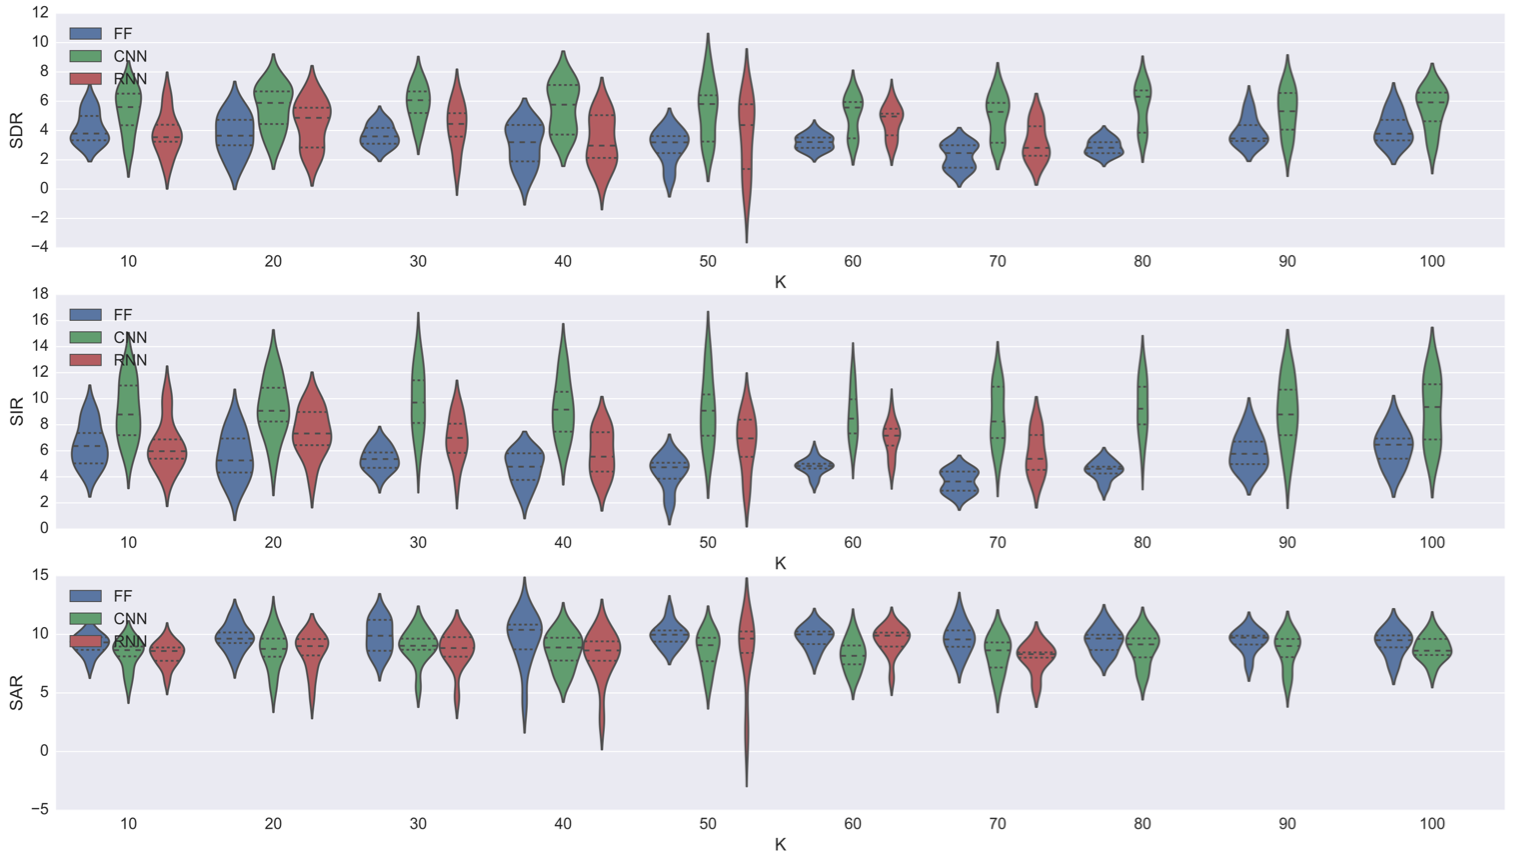
\includegraphics[clip, trim = 0cm 0cm 0cm 0cm, width=\linewidth]{Figs/FullPerformance.png}
  \caption{Separation performance of convolutive models obtained using a CNN-CNN Auto-encoder for varying values of $K$. }~\label{fig:cnnseparation_performance}
\end{figure*}

\section{Experiments}
\label{sec:experiments}
We now describe the experimental setup used to evaluate our auto-encoder based convolutive audio models. We construct a set of training and test examples using the TIMIT corpus~\cite{timit} for the evaluation. To form the examples, we randomly select a pair of male-female speakers from the TIMIT corpus. Of the $10$ utterances available for each speaker, one utterance is randomly selected for each speaker. These two selected utterances are mixed at $0~dB$ to generate the testing mixture. The remaining $9$ utterances are used as training data to construct models for the sources. In other words, these examples are used to train the respective (convolutional/ feed-forward) auto-encoders. For the evaluation, we generate $20$ such mixtures and compare the models for different parameter configurations. As a pre-processing step, we apply a $1024$ point short-time Fourier transform representation with a hop of $25\%$. The magnitude spectrogram is then given as an input to the network. 

The neural networks are initialized using the Xavier initialization scheme~\cite{glorot2010understanding}. The networks are trained by applying a batch gradient descent training procedure and the parameters updated using the RMSProp algorithm~\cite{tieleman2012rmsprop}, with a learning rate and momentum of $0.001$ and $0.7$ respectively.

The CNN filters are selected to be $512$-point tall and $8$-point wide. Thus, the convolutions are performed only along the time axis. The number of CNN filters also decides the number of components in the decomposition. We evaluate these models over a varying number of CNN filters ranging from $10$ to $100$ uniformly in steps of $10$. We compare the separation performance in terms of median BSS\_eval metrics~\cite{fevotte2005bss_eval} viz., signal-to-distortion (SDR), signal-to-interference (SIR) and signal-to-artifact ratio (SAR) parameters.

\subsection{Results and Discussion}
\label{subsec:results}
Figure~\ref{fig:cnnseparation_performance} gives the separation performance for the CNN-CNN models (left) and RNN-CNN models (right) for varying values of number of filters~$K$. We evaluate the proposed CAE models by comparing the separation performance to their equivalent feed-forward~(FF) counterparts proposed in~\cite{smaragdis2017aneural}. In order to maintain a uniform experimental setup, we apply the separation scheme described in~\ref{sec:ss} to all the models. We plot the results in terms of a violin plot that also indicates the median value and the corresponding inter-quartile range for each $K$.

We see that the CAE models significantly out-perform their corresponding FF versions. This can be seen from the fact that the inter-quartile range in SDR for CAE models is higher than the inter-quartile range of corresponding FF models for several values of $K$. This improvement is a consequence of reduced interference generated by these models in source separation (See SIR plots). Although the SAR for CAE models degrades slightly as compared to FF models, the improvement in significant improvement in SIR compensates for this loss. The performance of the models achieves a peak value for $K=80$. However, the separation performance does not degrade significantly for other values of $K$. Thus, the choice of $K$ does not appear to be a very critical consideration for these models.

The convolutive speech models obtained by training the RCAE also outperform the FF auto-encoder models, as seen by the median values and inter-quartile ranges. This improvement in performance is not as pronounced as the CAE models for the case of speech mixtures. However, the experimentation serves as a proof of concept that exploring non-uniform auto-encoder architectures could lead to interesting and potentially powerful algorithms for several applications.  

\section{Conclusion}
\label{sec:conclusion}
In this paper, we developed and investigated the use of a convolutional auto-encoder as an alternative to learn convolutive basis decompositions of speech and audio signals. The ability of the networks to include temporal dependencies allow the auto-encoders to learn cross-frame structures in the input spectrogram. We demonstrated that this results in a significant improvement in separation performance as compared to feed-forward auto-encoder models. This approach also allows for several extensions and generalizations to convolutive audio models, that can be easily implemented using the available diversity of neural networks. One such extension considered in this paper is the use of auto-encoders formed by a cascade of recurrent and convolutive layers. Although these models are not as potent as CAE models for separation of speech mixtures, these extensions could lead to interesting non-uniform auto-encoder architectures for several applications.

% References should be produced using the bibtex program from suitable
% BiBTeX files (here: strings, refs, manuals). The IEEEbib.bst bibliography
% style file from IEEE produces unsorted bibliography list.
% -------------------------------------------------------------------------
\bibliographystyle{IEEEbib}
\bibliography{refs.bib}

\end{document}
